\section{CNNs for Image Classification}

当我们分析一个CNN的结构时,需要考虑以下的方面:

\begin{enumerate}
	\item 表示能力
	\item 是否适合任务
	\item 是否容易优化
	\item 代价
\end{enumerate}

\subsection{Reception Field}

如图,使用三层3*3卷积层,感受野与一层7*7卷积层相同.

\begin{figure}[htbp]
	\centering
	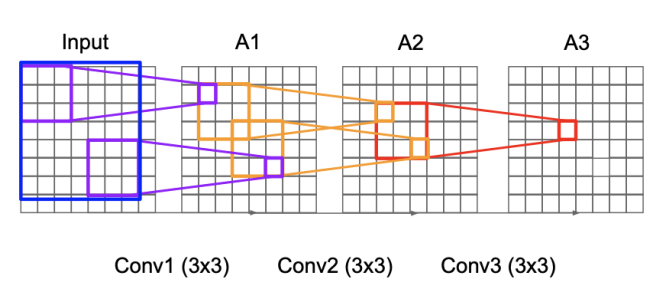
\includegraphics[scale=0.85]{figures/receptivefield.png}
	\caption{三层3*3卷积核的感受野}
\end{figure}

感受野是一个很重要的概念,它表征一个数据可以接收到原图多大范围的信息.
我们这里姑且认为感受野相同则表达能力相同.我们希望可以在神经网络的中部将整个图片纳入感受野,
这样在后面可以进行全图的pixel信息的交流,有利于结合多个特征.例如:结合狗的耳朵和毛色进行判断.

既然三层3*3卷积层,感受野与一层7*7卷积层相同,那么为什么要选用小而深的网络呢?
其一,层数增加,网络的非线性性增加,分割能力更强.此外,参数量也更小 ($3\times 3^2 C^2 < 7^2C^2$).